\documentclass{article}

\usepackage{graphicx}
\usepackage{amsmath}
\usepackage{lipsum}
\usepackage{multicol,caption}
\usepackage{fullpage}
\usepackage{url}
\usepackage{tabularx}
\usepackage{tabu}

\newenvironment{Figure}
  {\par\medskip\noindent\minipage{\linewidth}}
  {\endminipage\par\medskip}

\begin{document}

\title{Numerical Solutions of the Lippmann-Schwinger Equation for Simple NN Potentials -- Report for Project \#1}
\author{Dillon Frame, Hao Lin, Han Liu}
\date{\today}

\maketitle

\begin{abstract}
In this first project, we are interested in solving the Lipmann-Schwinger equation for a system of two nucleons interacting with a simple potential. We work in momentum space, and compute the $^1S_0$ phase shift as a function of center-of-mass energy by evaluating the reaction matrix ("R-Matrix"). We also investigated the Variable Phase Approach (VPA) as an alternative means for calculating the phase shifts, and its relation to the Levinson's theorem in determining the number of bound states a potential supports.
\end{abstract}

\begin{multicols}{2}

\section{Introduction}

This first project was broken into four parts. In this section, we will describe the goal of each part and give a brief overview of what our implementation for each part was. More detail will be provided in Section 2.

In Section 3, we will summarize our results for the $^1S_0$ phase shifts calculated with our C++ programs, and show comparisons with the NN-OnLine database of Nijmegen [2]. Additionally, we will make observations about the physics we can extract from the phase shift data. 

In Section 4, we will show a number of theoretical results obtained from the Variable Phase Approach (VPA), including the derivation of the analytic phase shifts for an attractive square well potential, the relationship between the sign of the phase shifts and the sign of the potential, and a sketch of the proof of the Levinson's Theorem from VPA.

Finally, in Section 5, we will summarize everything that we did in this project, as well as what we learned. We will also provide an outlook about possible extensions to either multi-channel systems, or more realistic nuclear potentials.

\section{Methods}

In this section, we provide a more detailed description of each part of the project. Additional details can be found in [1].

\subsection{Part 1a: Setting up the integration domain, mesh points and weights}

For this part, we wanted to set up our numerical integration by using a Gaussian Quadrature technique, using Legendre polynomials as our expansion functions.

We used the provided C++ function \textit{GaussLegendreQuadrature}(a,b,x[],w[],N) from the course website to generate our mesh points and weights in position space, on the interval $ x \in [-1,1]$. We needed to map these to mesh points and weights in momentum space using
\begin{equation*}
          k_i=const\times tan\left\{\frac{\pi}{4}(1+x_i)\right\},
        \end{equation*}
and

\begin{equation*}
            \omega_i= const\frac{\pi}{4}\frac{w_i}{cos^2\left(\frac{\pi}{4}(1+x_i)\right)}.
\end{equation*}
$const$ = 1 when the unit of $k$ is chosen to be fm$^{-1}$. 

\subsection{Part 1b: Adding a potential model}

To simulate the NN Interaction, we needed to introduce an interaction potential to use in the Lippmann-Schwinger Equation. For this, we used a simple, phenomenological potential defined by three parameterized, Yukawa-like terms:

\begin{equation}
V(R) = V_a\frac{e^{-a\mu R}}{\mu R} + V_b\frac{e^{-b\mu R}}{\mu R} + V_c\frac{e^{-c\mu R}}{\mu R}
\end{equation}

\noindent with $R = |r-r'|$, $\mu = 137 $ MeV (or $0.7$ fm$^{-1}$), $a = 1$, $b = 4$, $c = 7$, $V_a = -10.463$ MeV, $V_b = -1650.6$ MeV, and $V_c = 6484.3$ MeV.

Since we wish to work in momentum space, we need to perform a Fourier Transform of this potential. It will also be a simplification if we absorb the $\mu$ into the definitions for each parameter.

For a potential of the form

\begin{equation}
V(R) = V_0\frac{e^{-\mu R}}{R}
\end{equation}

the Fourier transform is given by

\begin{equation}
V(k_1,k_2) = \frac{V_0}{4\mu k_1 k_2}\ln{\left[\frac{\left(k_1 + k_2\right)^2 + \mu^2}{\left(k_1 - k_2\right)^2 + \mu^2}\right]}
\end{equation}

Since the Fourier Transform is a linear operation, we can generate the transform of Eq. (1) by transforming each term individually, and then adding them together.

In the two plots below, we show the values of the potential for the mesh points generated by the \textit{GaussLegendreQuadrature} subroutine, and for the raw index values of the potential matrix V.

\begin{Figure}
\centering
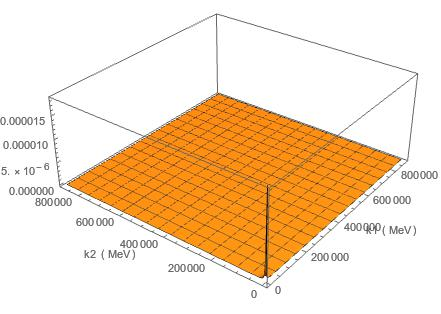
\includegraphics[width=\textwidth]{potential_real.jpeg}
\captionof{figure}{Potential Energy Function in Momentum Space, using the actual values for $k_1$ and $k_2$. Note the delta function like structure near the origin, and otherwise boring structure.}
\end{Figure}

\begin{Figure}
\centering
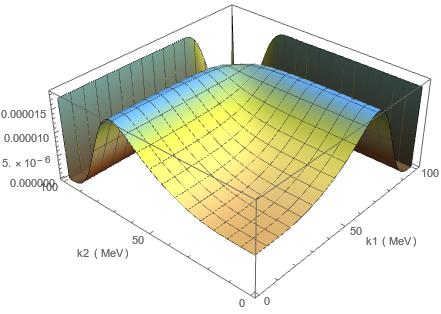
\includegraphics[width=\textwidth]{potential.jpeg}
\captionof{figure}{Potential Energy Function in Momentum Space. Labels on x-axis and y-axis are index labels for the array, so do not correspond with the actual values of $k_1$ and $k_2$}
\end{Figure}

\subsection{Part 1c: Handling the Principal Value Problem}

For this part, we needed to solve the Lippmann-Schwinger equation for $R(k,k^\prime)$. One issue regarding the principal value integral is that the integrand has a 2nd-order pole. This singularity can be removed though with a smart trick.

With simple calculus, it can be shown that the following relation holds
\begin{equation}
\int_{-\infty}^{+\infty} \frac{dk}{k^2-k_0^2}=0,
\end{equation}
which can be used to rewrite principal value integrals with a 2nd-order pole in general
\begin{equation}
	\mathcal{P}\int_0^{\infty} \frac{f(k)dk}{k^2-k_0^2} = \int_0^{\infty} \frac{(f(k)-f(k_0))dk}{k^2-k_0^2}.
\end{equation}

Upon applying this trick to the Lippmann-Schwinger equation discretized in momentum space, we have
\begin{equation}
\begin{split}
    R(k,k') &= V(k,k') +\frac{2}{\pi} \cdot \\
                &\int_0^{\infty}dq
                \frac{q^2V(k,q)R(q,k')-k_0^2V(k,k_0)R(k_0,k')  }
                     {(k_0^2-q^2)/m} \\
               &= V(k,k') +\frac{2}{\pi}\sum_{j=1}^N\frac{\omega_jk_j^2V(k,k_j)R(k_j,k')}{(k_0^2-k_j^2)/m} \\
               &-\frac{2}{\pi}k_0^2V(k,k_0)R(k_0,k')\sum_{n=1}^N\frac{\omega_n}{(k_0^2-k_n^2)/m}.
\end{split}
\end{equation}

The discretized form of Eq. (6) can be identified as a matrix equation $A_{i,l}R_{l,j}=V_{i,j}$ with a proper definition of the matrix $A$
\begin{equation}        \label{eq:aeq}
A_{i,j}=\delta_{i,j}-V(k_i,k_j)u_j,
\end{equation}
where $\delta$ is the Kronecker $\delta$
and

\begin{equation}
     u_j=\frac{2}{\pi}
         \frac{\omega_jk_j^2}{(k_0^2-k_j^2)/m}\hspace{1cm}
         j=1,N
\end{equation}
and

\begin{equation}
     u_{N+1}=-\frac{2}{\pi}
          \sum_{j=1}^N\frac{k_0^2\omega_j}{(k_0^2-k_j^2)/m}.
\end{equation}

We can solve the matrix equation for $R$
\begin{equation} \label{eq:final2}
R=A^{-1}V.     
\end{equation}
In the end, the phase-shift can be found using the following relation
\begin{equation}
R(k_{N+1},k_{N+1}) = R(k_0,k_0)=-\frac{tan\delta}{mk_0}.
\end{equation}

\section{Results of $^{1}S_{0}$ phase shifts}

In Figure 3, we show the calculated $^{1}S_{0}$ phase shift as a function of the center-of-mass kinetic energy. We performed the calculations with a varying number of mesh points. Phase shifts from calculations with 20, 50 and 100 mesh points turned out to be almost indistinguishable, confirming that we have used sufficiently fine meshes and obtained convergent results. The relatively small number of mesh points needed also demonstrates the efficiency of solving the discretized Lippmann-Schwinger equation with matrix inversion.

\begin{Figure}
\centering
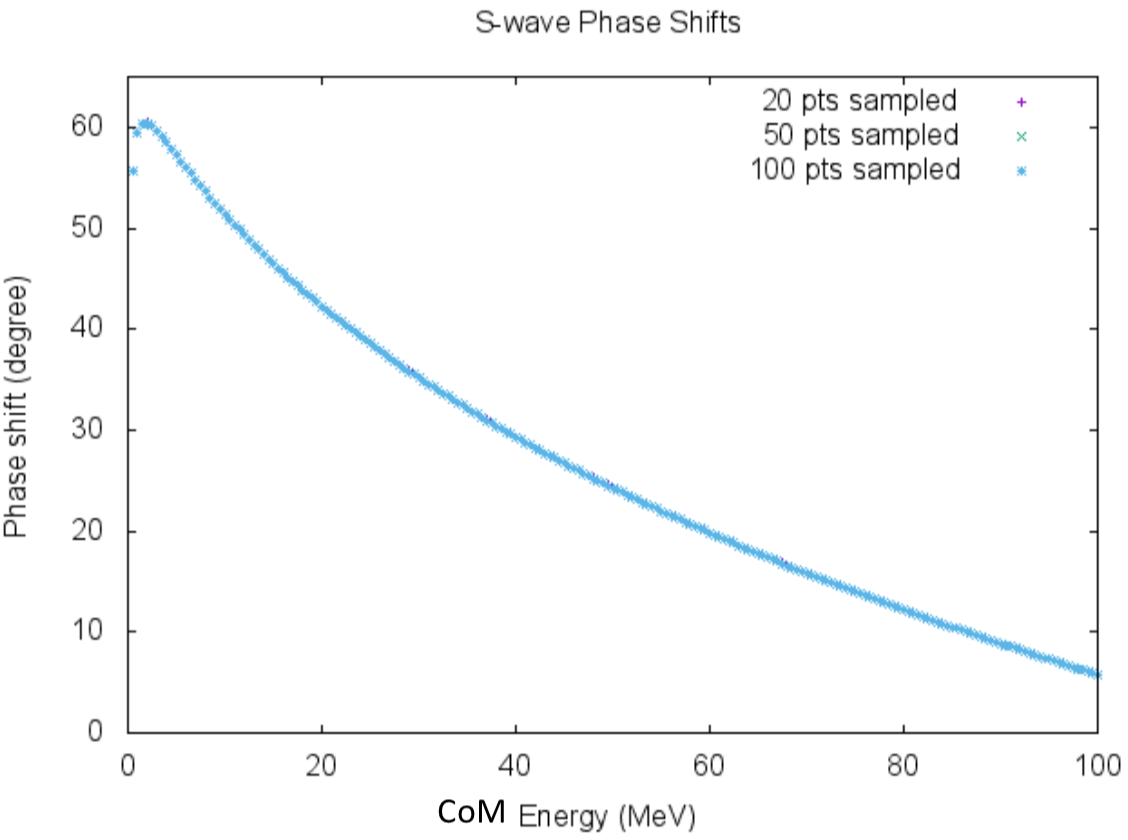
\includegraphics[width=0.95\textwidth]{delta_mesh.png}
\label{mesh}
\captionof{figure}{$^{1}S_{0}$ phase shift as a function of kinetic energy in the center of mass frame. Results from calculations using 20, 50 and 100 mesh points are shown.}
\end{Figure}

In addition to solving the Lippmann-Schwinger equation in momentum space, we were also able to carry out the calculations by directly solving the good-old Schr\"{o}dinger equation in position space and using the same NN interaction potential shown in Eq. (1). Calculations from both the Lippmann-Schwinger equation and the Schr\"{o}dinger equation are compared with those from the PWA93 and the NIJM93 models in Figure 4. 

\begin{Figure}
\centering
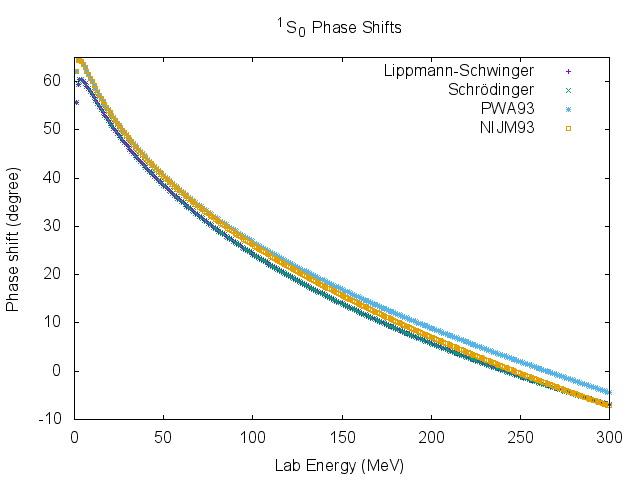
\includegraphics[width=\textwidth]{res.png}
\label{compare}
\captionof{figure}{$^{1}S_{0}$ phase shift as a function of kinetic energy in the lab frame. Result from solving the Lippmann-Schwinger equation is compared with calculatoins from the Schr\"{o}dinger equation, the PWA93 model and the NIJM93 model.}
\end{Figure}

Unsurprisingly, phase shifts from solutions of the Lippmann-Schwinger equation are identical to those of the Schr\"{o}dinger equation, indicating the theoretical equivalence of the two approaches. Numerically, the Lippmann-Schwinger approach appears more elegant and care-free, while there exists arbitrainess in the initial conditions for integrating the wave function outward from the origin in the Schr\"{o}dinger approach owing to the non-normalizability of the scattering wave functions.

Compared with the more sophisticated models such as PWA93 and NIJM93, our calculations show essentially the same pattern. Our results agree with the NIJM93 calculations reasonably well, with the exception of slight underestimates in the low energy regime. Note in particular that the phase shift at zero energy tends towards 0, and the peak of the phase shift is somewhat above 60 degrees located at around $E_{lab}$ = 4 MeV. It is now clear from the Levinson's theorem that the phenomenological nucleon-nucleon potential does not support any bound state with $l$ = 0. Also, the phase shift turns negative at around $E_{lab}$ = 250 MeV, from which we may conclude that the nucleon-nucleon interaction is attractive at low energies but repulsive at high energies. This can be understood from the fact that as the probing energy increases, the minimum distance between the two nucleons drops drastically which eventually gives rise to the hard sphere-like short-ranged repulsion.

\section{Variable Phase Approach (VPA)}
In this section, we first derived the analytic phase shifts for a square well potential, confirming the applicability of VPA. We then proceeded to investigate the relationship between phase shifts and potentials, and showed that a fully attractive potential yields positive s-wave phase shifts while a fully negative potential gives negative s-wave phase shifts. In the end, we sketched a convincing argument for the Levinson's theorem based on the variable phase approach in the special case of $l$ = 0. 

The work was done with pen and paper. Time limiting, we have yet to digitalize it. Please kindly refer to the attached \emph{handwritten} notes for more details.


\clearpage
\section{Conclusion}
Numerical methods were used to solve the Lipmann-Schwinger equation with a given simple NN potential for $^1S_0$ wave. The convergence of the numerical methods was explored and it was shown the number of mesh points we chose was sufficient. The phase shifts were draw against lab energy and compared with the other calculations. Both qualitatively and quantitatively good agreements were achieved between the chosen data sets and our calculations. Alternatively, variable phase approach was studied with $l=0$. Analytical solutions for square well were derived, and the relation between the sign of phase shifts and the sign of potentials was shown. Throughout the project, we learned the numerical techniques for integrating and solving integral equations and practiced the fundamentals of scattering theory. In this study, the NN potential is local and independent of $l$, and only s-wave phase shifts were obtained. In the future, we may include more sophisticated interactions such as the tensor force and the spin-orbit coupling into the NN potential. In that case, couplings between different angular momentum $l$ values would play an essential role and much richer physics can emerge. 

\end{multicols}

\hrulefill

\begin{enumerate} % References

\item S. Bogner and M. Hjorth-Jensen, \textit{Project 1 Assignment Notes}, \url{https://manybodyphysics.github.io/NuclearForces/doc/web/course.html}

\item NN-OnLine, Radboud University Nijmegen, \url{http://nn-online.org}

\end{enumerate}

\end{document}
